%======================================================================
\subsection{BW-PDM-04 --- Plan: the vault client in FreeCAD (23 Oct 2026, approved the same day, built 24 Oct)}\label{sec:pdm04-plan}
%======================================================================

\eref{PDM-04} brings the folder vault (\S\ref{sec:pdm-decision}) into FreeCAD. Today the vault can be made, filled
and configured from FreeCAD (the Create Vault, Import and Vault Settings task panels), but checking a file out and
in still needs the command line. This plan covers the rest of the epic: check out, check in, undo check-out, get
latest, get a revision, status everywhere, and links that resolve through the vault. The acceptance stays as written:
\emph{a check-out/check-in round trip of \code{LE-02001} from an iCloud Drive vault inside FreeCAD, with correct
status icons.} The scope is still \textbf{one FreeCAD at a time}. Approvals stay in \eref{PDM-05}.

\paragraph{Your answers (23 Oct).}
\begin{center}
\small
\begin{tabularx}{\linewidth}{@{}lX@{}}
\toprule
Question & Answer\\
\midrule
Revisions & Keep ASME Y14.35 (figure~\ref{fig:lifecycle-sm}): 01, 02 while in work, A at the first release, later
  letters only through ECR $\rightarrow$ ECO. The Create Vault panel no longer asks for a ``first revision'' and
  shows numbers without one (\code{BW-01-01001-001}).\\
Working files & \textbf{Inside the vault folder} (a change from 19 Oct, see below).\\
Vault in FreeCAD & All three: a Data panel, Browser badges and a right-click menu, the status bar and the Start page.\\
Links & Files are named by part number and links are rewritten to those names.\\
Start page & The left-hand vault box goes. A one-line vault switcher stays on the left; a \emph{My work} list
  joins the right-hand side.\\
\bottomrule
\end{tabularx}
\end{center}

\begin{figure}[!htbp]
\centering
\begin{tikzpicture}
  \node[anchor=south west,inner sep=0] (img) at (0,0) {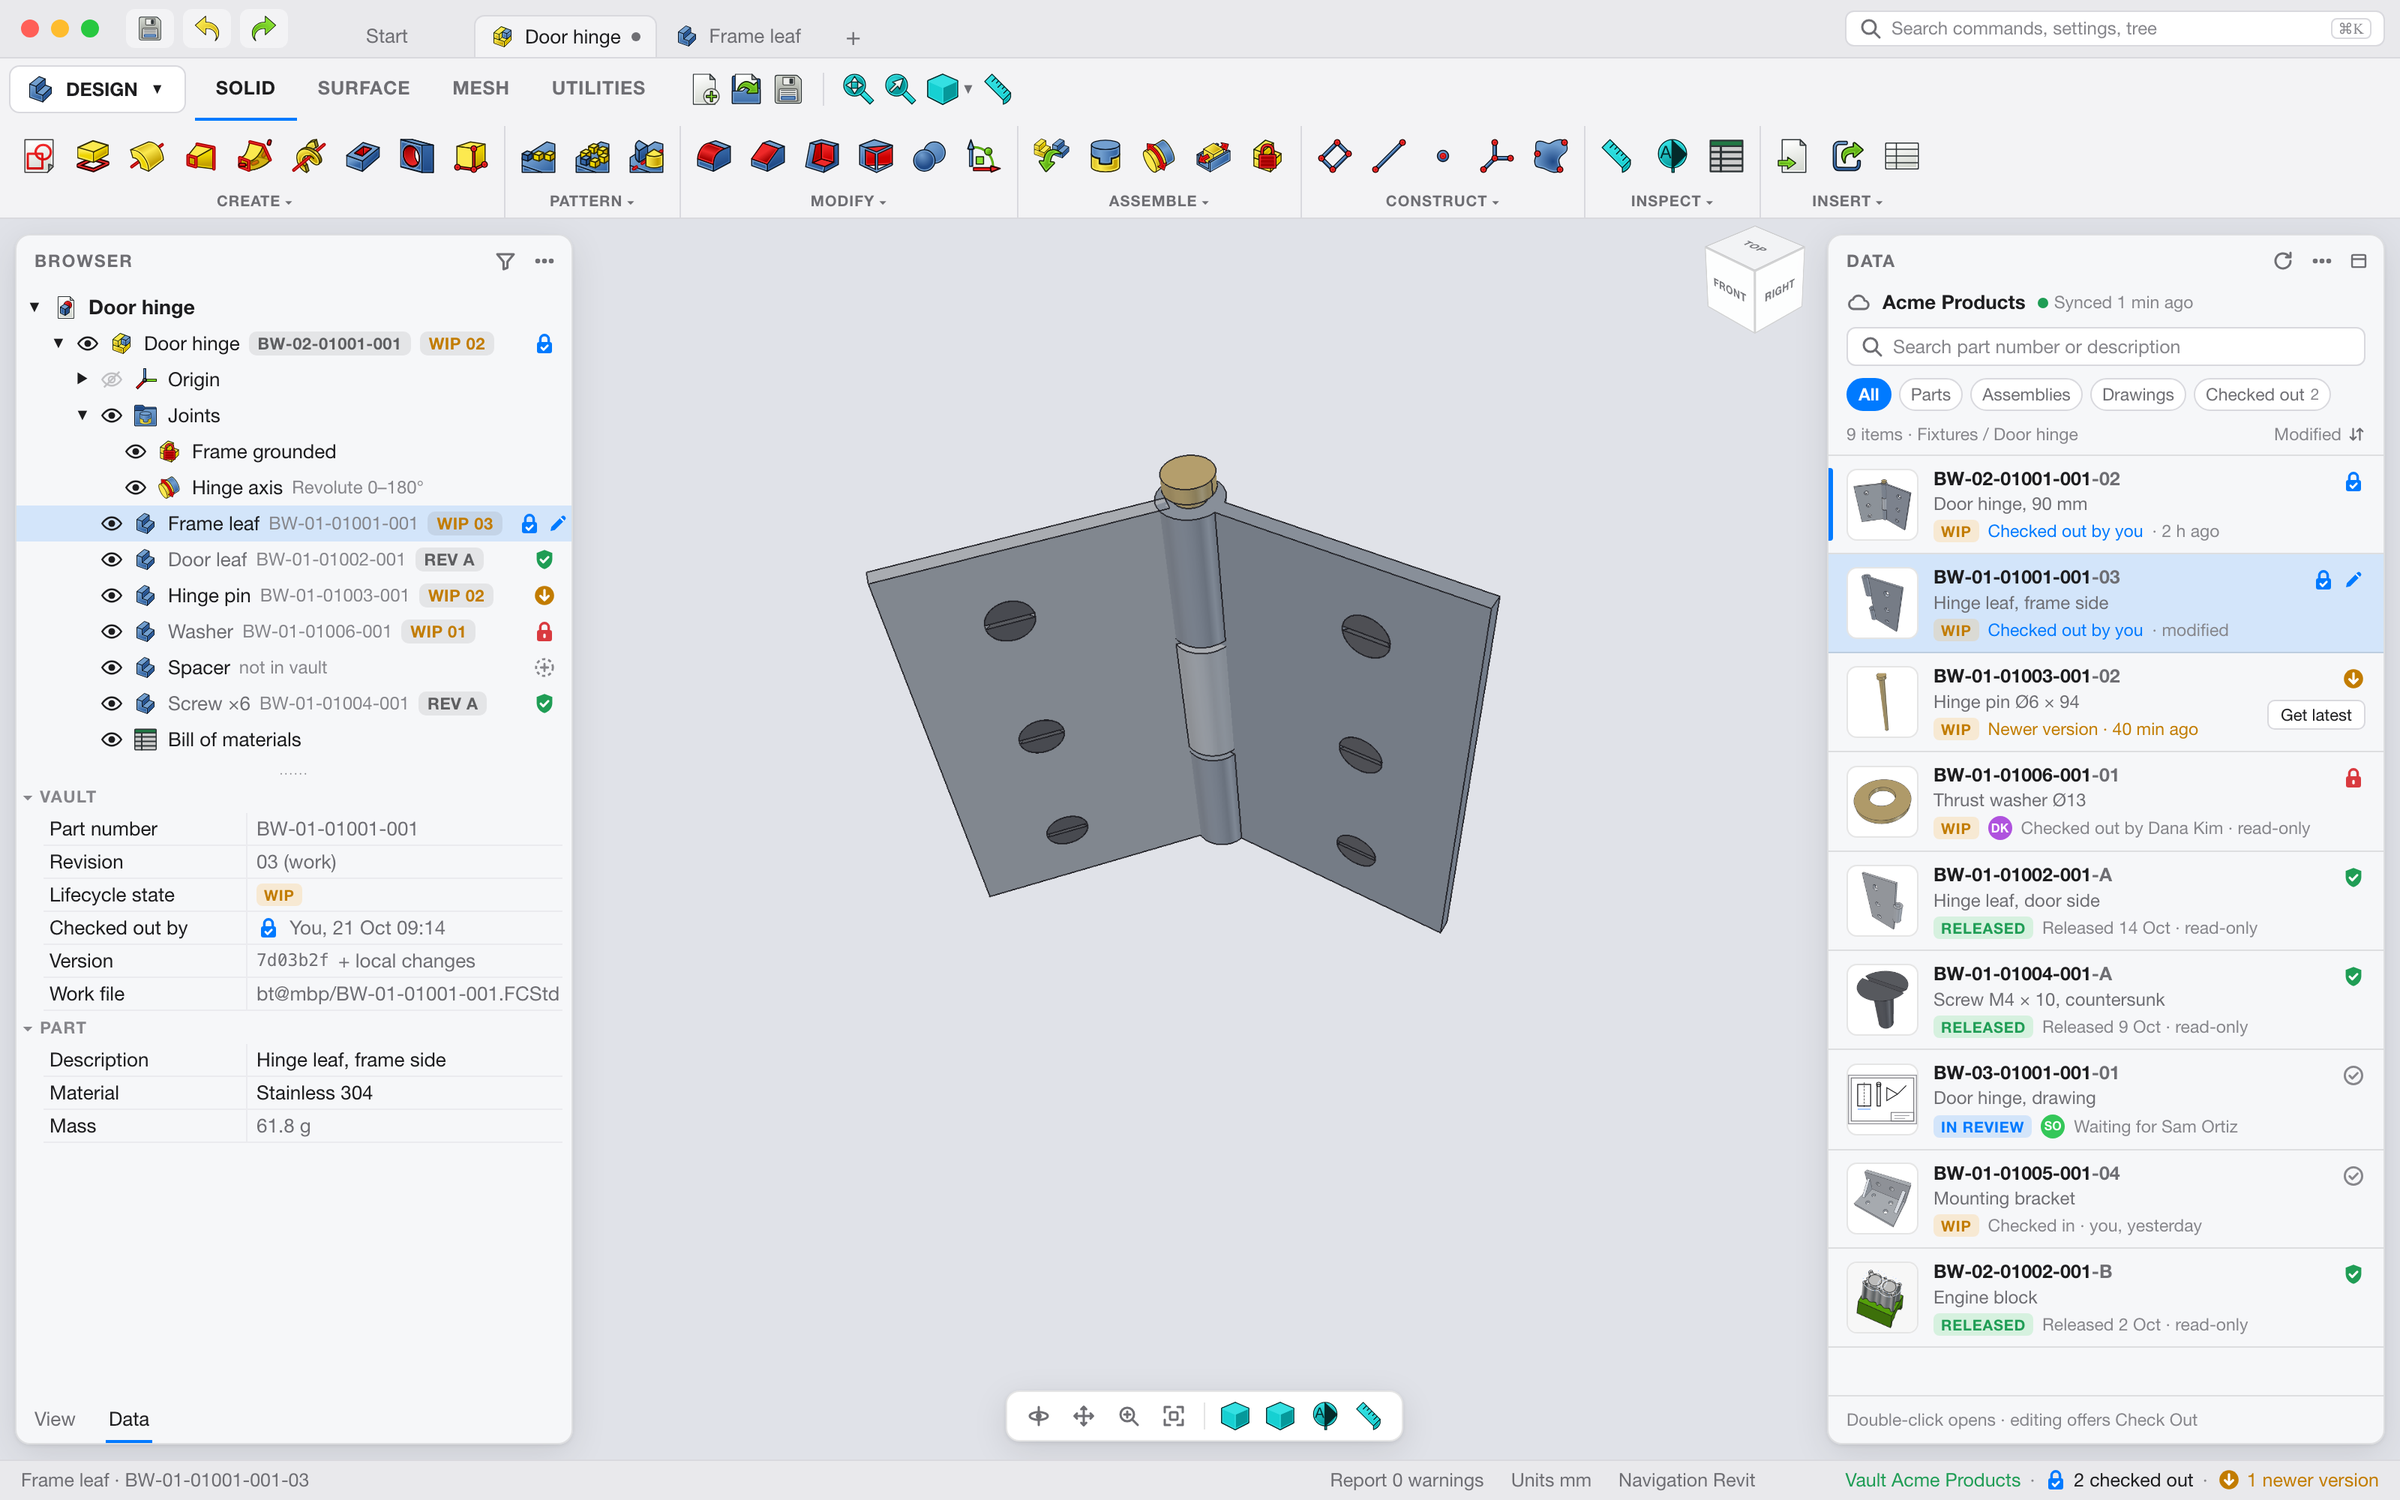
\includegraphics[width=\linewidth]{fig/pdm04_overview.png}};
  \begin{scope}[x={(img.south east)},y={(img.north west)}]
    \foreach \n/\x/\y in {1/0.245/0.651, 2/0.755/0.832, 3/0.753/0.016}
      \node[circle,fill=bwred,text=white,font=\tiny\bfseries,inner sep=0.6pt,minimum size=13pt,draw=white,line width=0.8pt] at (\x,\y) {\n};
  \end{scope}
\end{tikzpicture}
\caption{PDM-04 in the window (mock). \textbf{1}~Browser badges: revision and state per part, a lock while checked
out. \textbf{2}~The Data panel lists the vault. \textbf{3}~The status bar counts what is checked out and what is out
of date.}
\label{fig:pdm04-overview}
\end{figure}

%----------------------------------------------------------------------
\subsubsection*{1. Working files inside the vault}

\textbf{Layout.} One new folder per user and Mac, with the same rule as the journal: only its owner writes it.
\begin{center}
\small
\begin{tabularx}{\linewidth}{@{}lX@{}}
\toprule
Path & Holds\\
\midrule
\file{work/<user>@<mac>/<P/N>.FCStd} & The files you work on: the ones checked out to you (writable) and the
  read-only copies of what they link to.\\
\file{work/<user>@<mac>/.bw/state.json} & For each file there: the vault version it started from (its SHA-256,
  the \emph{base}), when it was fetched, and whether it is checked out.\\
\file{work/<user>@<mac>/.rev/<P/N>-<rev>.FCStd} & Older revisions fetched with \emph{Get revision}, read-only.\\
\bottomrule
\end{tabularx}
\end{center}

\textbf{What changes against 19 Oct, and why it is still safe.} On 19 Oct the working folder was outside the vault,
so that saving every few minutes never touched iCloud. Inside the vault, iCloud uploads every save. That is
traffic, not risk: a sync service makes conflict copies only when \emph{the same file} changes on two Macs, and
\file{work/<user>@<mac>/} is written by one Mac only. Three things need handling:
\begin{itemize}[nosep]
  \item \emph{Backups.} FreeCAD writes \file{.FCBak} files next to a saved file. In the vault they would be synced
        too. The client keeps them, but in \file{work/<user>@<mac>/.bw/backup/}, and limits them to one per file
        (question~4).
  \item \emph{Optimise Mac Storage.} iCloud may remove the local copy of a file nobody opened for a while. Before
        opening a file the client asks for it to be downloaded and waits (\verify: the call is
        \code{NSFileManager startDownloadingUbiquitousItemAtURL}, reachable from \code{ctypes} as in C4).
  \item \emph{A half-uploaded save.} The vault only reads \file{objects/} and \file{journal/}, which are written
        once; a work file in transit is never read by another Mac.
\end{itemize}
Vault Settings keeps a switch \emph{Working files outside the vault} for later, should the traffic matter.

%----------------------------------------------------------------------
\subsubsection*{2. Theory: the status of a file}

Every status icon follows from five facts about an item $p$, all cheap to know:
\[
\begin{aligned}
L(p) &\in \{\varnothing, \text{me}, \text{other}\} && \text{who holds the lock (journal)}\\
v(p) &= \text{SHA-256 of the latest vault version} && \text{(journal)}\\
b(p) &= \text{SHA-256 the work copy started from} && \text{(\file{state.json})}\\
w(p) &= \text{SHA-256 of the work copy, or } \varnothing && \text{(file, cached by size and mtime)}\\
s(p) &\in \{\text{WIP}, \text{In Review}, \text{Released}, \text{Obsolete}\} && \text{(journal)}
\end{aligned}
\]
The status is the first row of this table that holds:
\begin{center}
\small
\begin{tabular}{@{}lll@{}}
\toprule
Condition & Status & File\\
\midrule
$p$ not in the vault & Not in vault & as is\\
$L = \text{other}$ & Checked out by someone else & read-only\\
$L = \text{me},\ w \ne b$ & Checked out to me, modified & writable\\
$L = \text{me}$ & Checked out to me & writable\\
$w \ne \varnothing,\ b \ne v$ & Newer version in the vault & read-only\\
$s = \text{Released}$ & Released & read-only\\
otherwise & Checked in, up to date & read-only\\
\bottomrule
\end{tabular}
\end{center}
Hashing a 20\,MB file takes about 20\,ms, and the hash is cached by (size, mtime), so the Browser and the Data panel
can show the status of every file without slowing down. ``Modified'' compares content, not dates: saving without a
change leaves a file unmodified.

\begin{figure}[!htbp]
\centering
\IfFileExists{fig/pdm04_states.png}{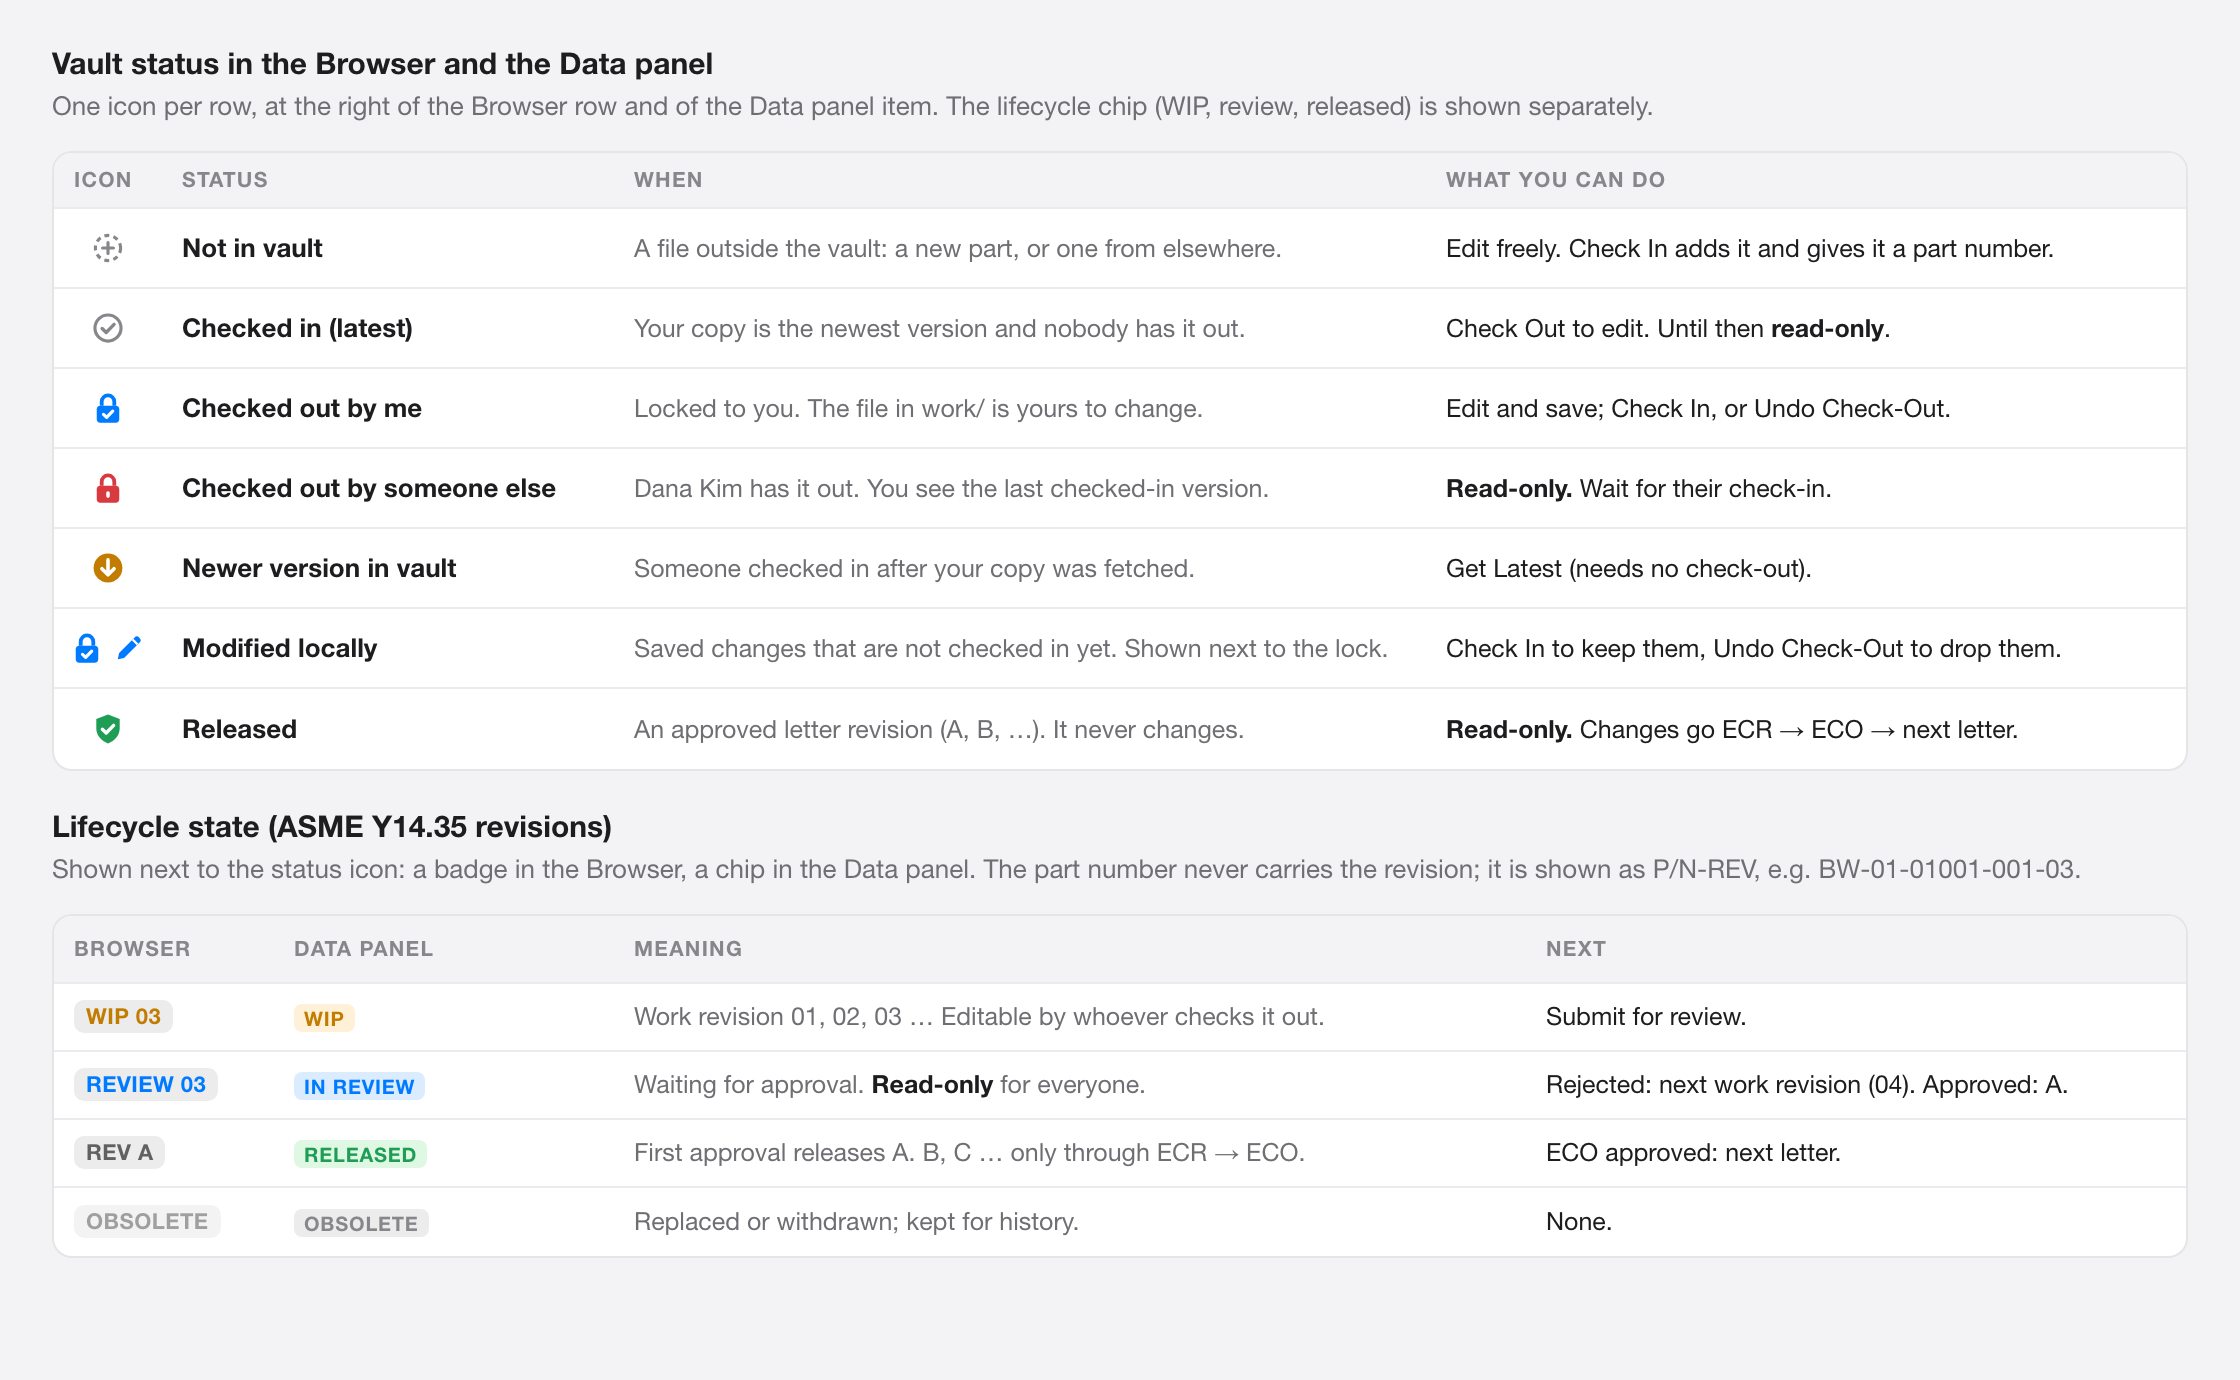
\includegraphics[width=0.8\linewidth]{fig/pdm04_states.png}}{\fbox{pdm04\_states.png}}
\caption{The status icons (mock), one per row of the table above.}
\label{fig:pdm04-states}
\end{figure}

%----------------------------------------------------------------------
\subsubsection*{3. Operations}

\begin{itemize}[nosep]
  \item \textbf{Check out.} Takes the lock (journal), copies the latest version to \file{work/.../<P/N>.FCStd},
        makes it writable and records the base. For an assembly it also fetches what it links to, read-only, so
        it opens complete (question~1).
  \item \textbf{Check in\ldots} opens a task panel (figure~\ref{fig:pdm04-checkin}): a comment, the files that
        will go in (the assembly and the changed parts it links that are checked out to you), and \emph{keep
        checked out}. Unchanged files ($w = b$) are skipped. Links are rewritten (\S4) before the file is
        written to \file{objects/}. The lock is released and the file turns read-only.
  \item \textbf{Undo check-out} puts the base back after a confirmation (``discard 3 hours of changes?'') and
        releases the lock.
  \item \textbf{Get latest} replaces a read-only work copy with the latest version, and reloads it if it is open.
        A file checked out to you is never overwritten.
  \item \textbf{Get revision\ldots} fetches an older version into \file{.rev/}, read-only.
  \item \textbf{Saving a file that is not checked out.} Vault files that are not checked out to you are
        read-only on disk. FreeCAD tells Python when a save starts (\code{slotStartSaveDocument}), before it
        writes. The client then asks ``Check out \code{BW-01-01001-001} to save?''. \emph{Yes} takes the lock and
        makes the file writable in time for the save; \emph{No} lets FreeCAD's save fail with its normal message,
        and the document stays open and unchanged (\verify).
  \item \textbf{Opening a vault file} that is not checked out opens the read-only copy; its tab and the task card
        show a lock, and the first edit offers a check-out.
  \item \textbf{Move vault\ldots} (your request, 23 Oct), in Vault Settings: moves the whole vault, say to an SSD.
        The vault is \emph{copied} into \file{<name>.moving}, every file is compared by SHA-256, the copy is opened and
        must replay to the same items, versions and locks, and only then is it renamed into place
        (\file{bruceworx/vault\_move.py}). FreeCAD then switches to the new place and reopens your documents from
        there; the old copy goes to the Trash only if you say so. A move is refused when there is not enough space,
        the destination is inside the vault or not empty, or files have not finished downloading from iCloud.
\end{itemize}

\begin{figure}[!htbp]
\centering
\IfFileExists{fig/pdm04_checkin.png}{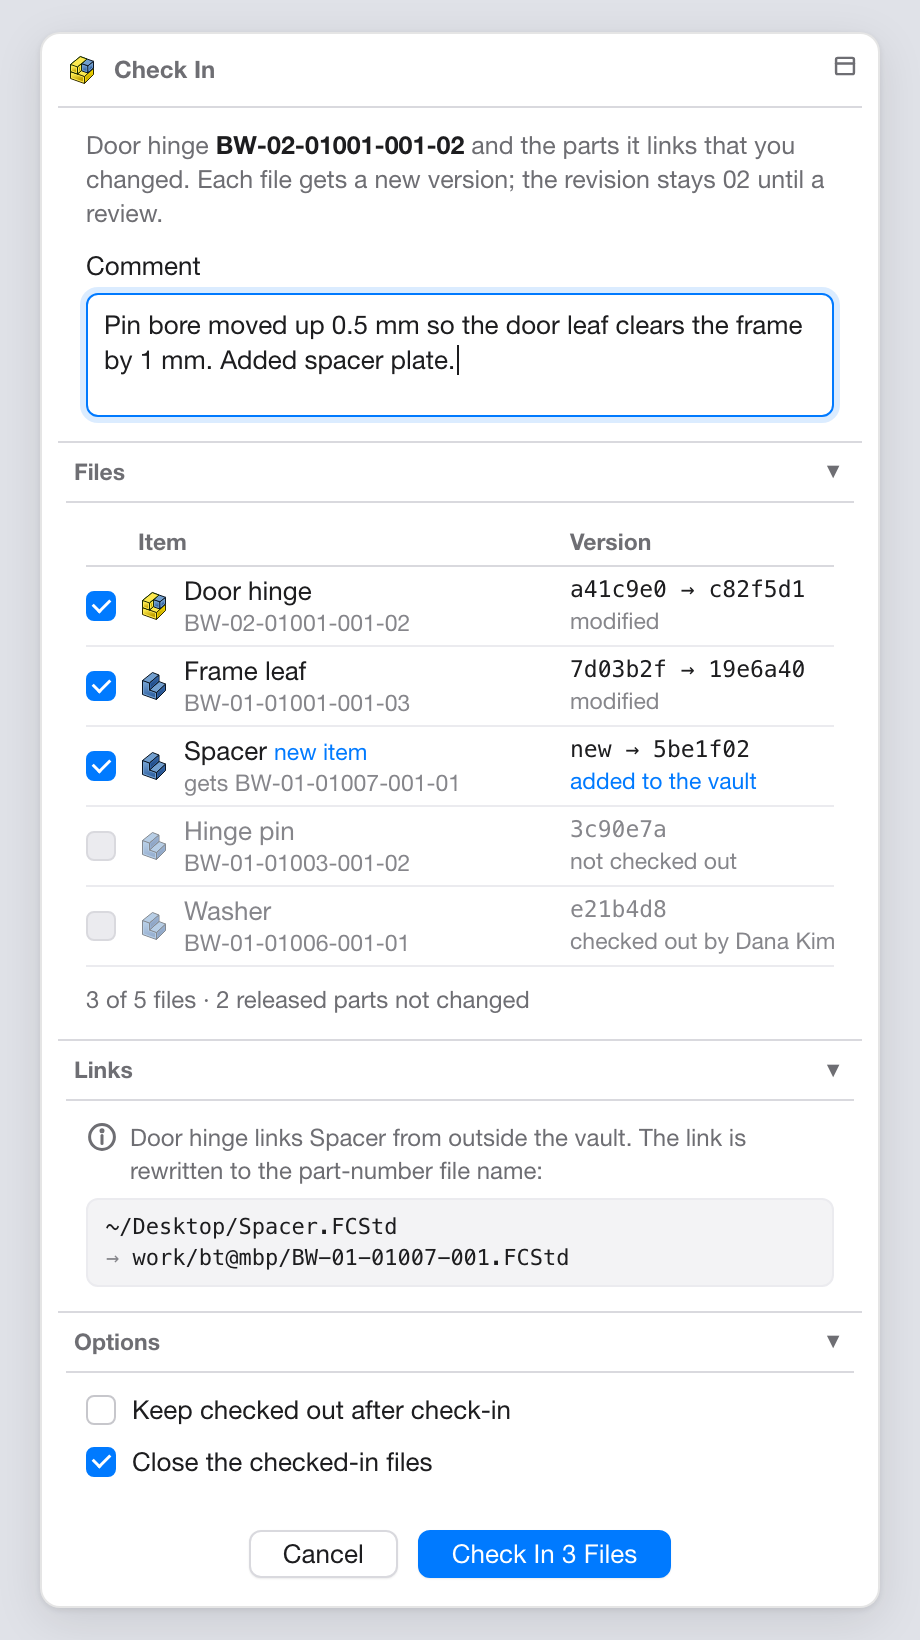
\includegraphics[height=8.5cm]{fig/pdm04_checkin.png}}{\fbox{pdm04\_checkin.png}}\hspace{6mm}
\IfFileExists{fig/pdm04_contextmenu.png}{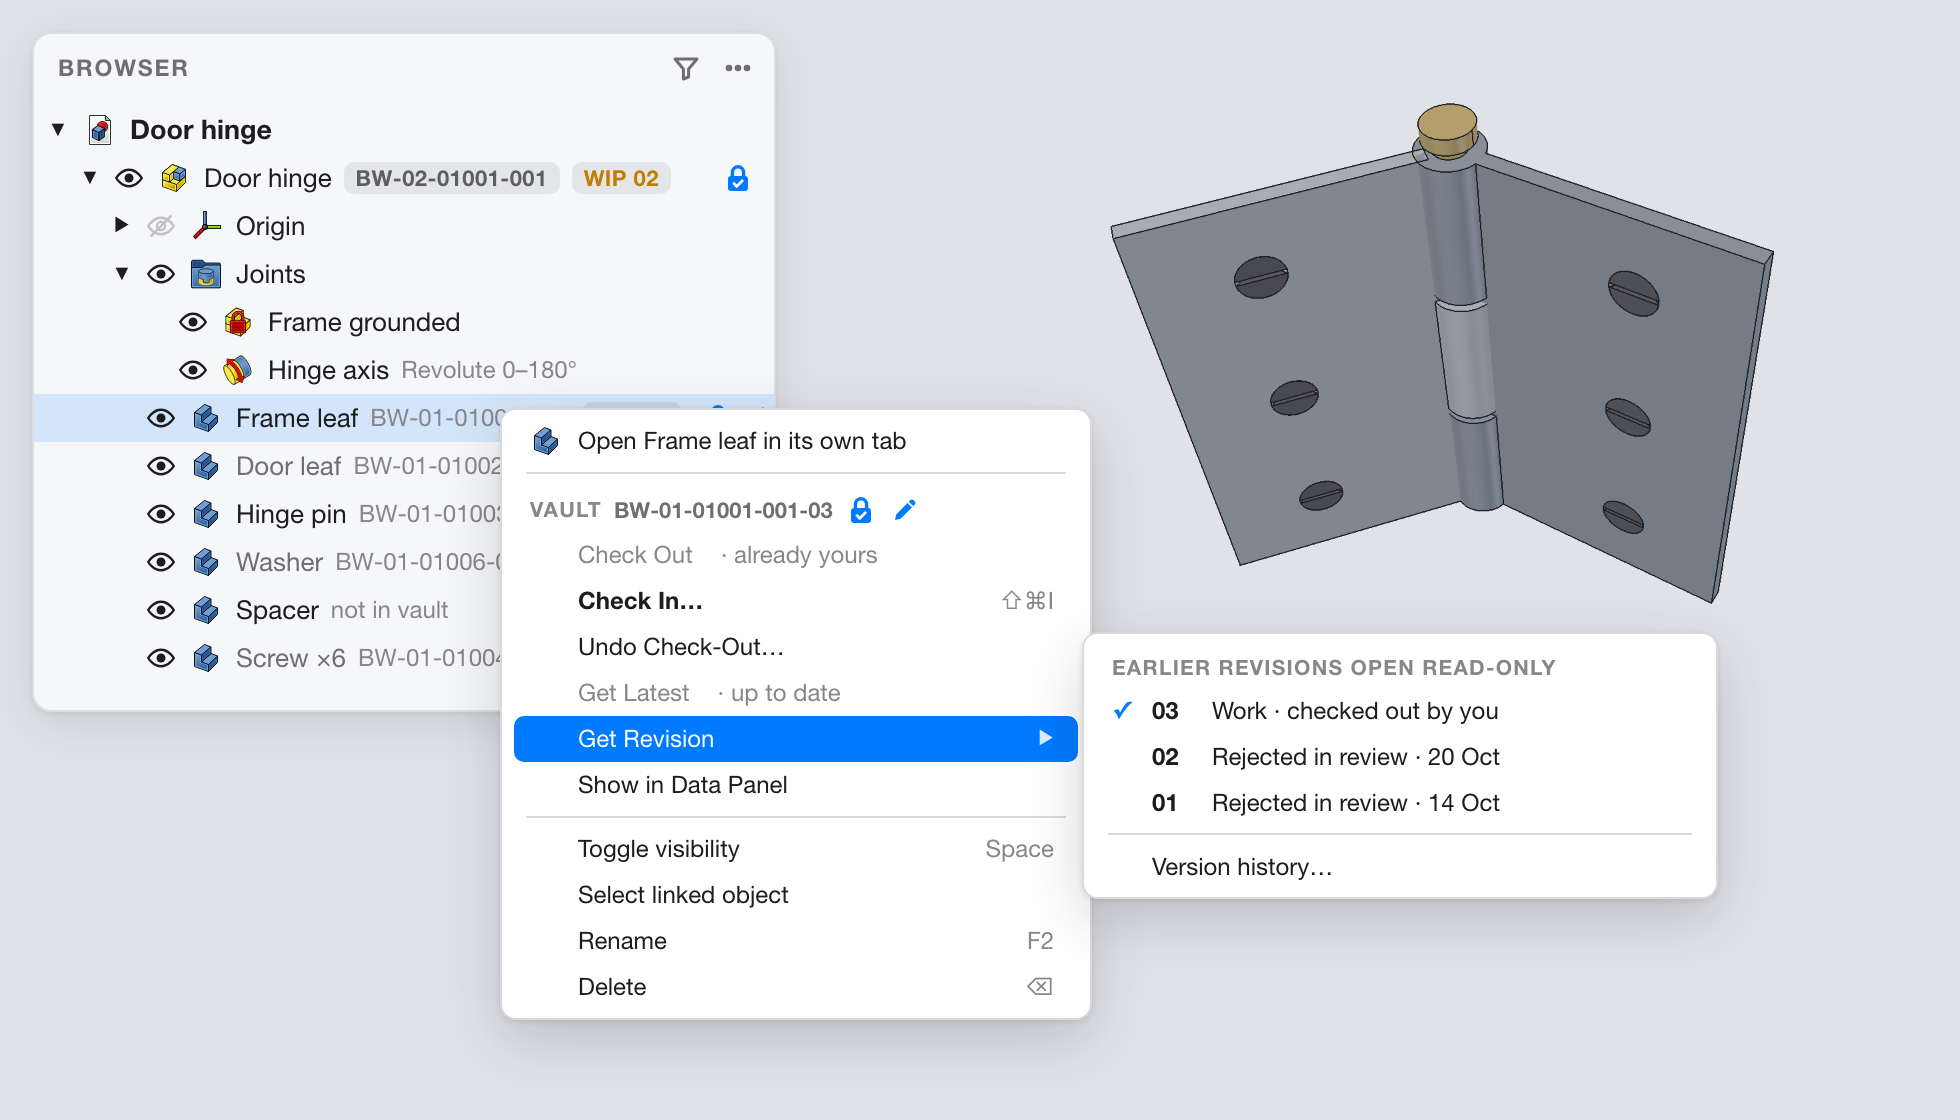
\includegraphics[height=8.5cm]{fig/pdm04_contextmenu.png}}{\fbox{pdm04\_contextmenu.png}}
\caption{\emph{Left:} the Check In task panel (mock). \emph{Right:} the Browser's right-click menu on a part
(mock).}
\label{fig:pdm04-checkin}
\end{figure}

%----------------------------------------------------------------------
\subsubsection*{4. Links that resolve through the vault}

FreeCAD stores a link to another file as \code{<XLink file="..." ...>} in \file{Document.xml}
(\file{App/PropertyLinks.cpp:4184}) and looks for that path relative to the document first. If every work file is
called \file{<P/N>.FCStd} and sits in the same folder, a link whose path is just \file{<P/N>.FCStd} resolves on every
Mac. So:
\begin{itemize}[nosep]
  \item \textbf{On import} the vault already knows which original file became which part number. The import
        rewrites each \code{file} attribute in the copies through that map, in the zip, without FreeCAD.
  \item \textbf{On check-in} the same rewrite runs for links that still point outside the work folder (a part
        added from elsewhere): a file that is not in the vault yet is offered for import first.
  \item \textbf{On check-out} the linked items are fetched (transitively) so the assembly opens complete.
\end{itemize}
This is also the acceptance of \eref{ASM-01}: \code{LE-02001} opens from a moved folder with no broken links.
Theory: the link graph is a DAG over items; fetching the closure is a depth-first walk with a visited set,
$O(\text{items} + \text{links})$, and a cycle (which FreeCAD allows between files) stops at the visited set.

%----------------------------------------------------------------------
\subsubsection*{5. In the window}

\begin{itemize}[nosep]
  \item \textbf{Data panel} (figure~\ref{fig:pdm04-data}). A floating card on the right, like the Browser on the
        left, opened from the status bar, View $\rightarrow$ Panels or \texttt{Cmd-K} ``Data''. It lists the vault's
        items with thumbnail, P/N, description, revision, state and lock, has a search field and filters (All,
        Parts, Assemblies, Drawings, Checked out), and the same right-click menu as the Browser. Double-click
        opens. It refreshes when the journal changes (\code{QFileSystemWatcher} on \file{journal/}).
  \item \textbf{Browser.} Next to the existing P/N badges (\file{bruceworx\_browser.py}): the revision and state
        chip, and a lock. Right-click: Check out, Check in\ldots, Undo check-out, Get latest, Get revision\ldots,
        Show in Data panel (a workbench manipulator, \code{modifyContextMenu}).
  \item \textbf{Status bar.} ``Vault Acme Products $\cdot$ 2 checked out $\cdot$ 1 newer''; a click opens the Data
        panel.
  \item \textbf{Start page.} The vault box on the left becomes one line, the vault's name with a menu (Open,
        Create, Settings, Import, Close vault). On the right, \emph{My work} comes above \emph{Recent}: files
        checked out to me, waiting for my review, and newer versions, as rows that open the file.
\end{itemize}

\begin{figure}[!htbp]
\centering
\IfFileExists{fig/pdm04_datapanel.png}{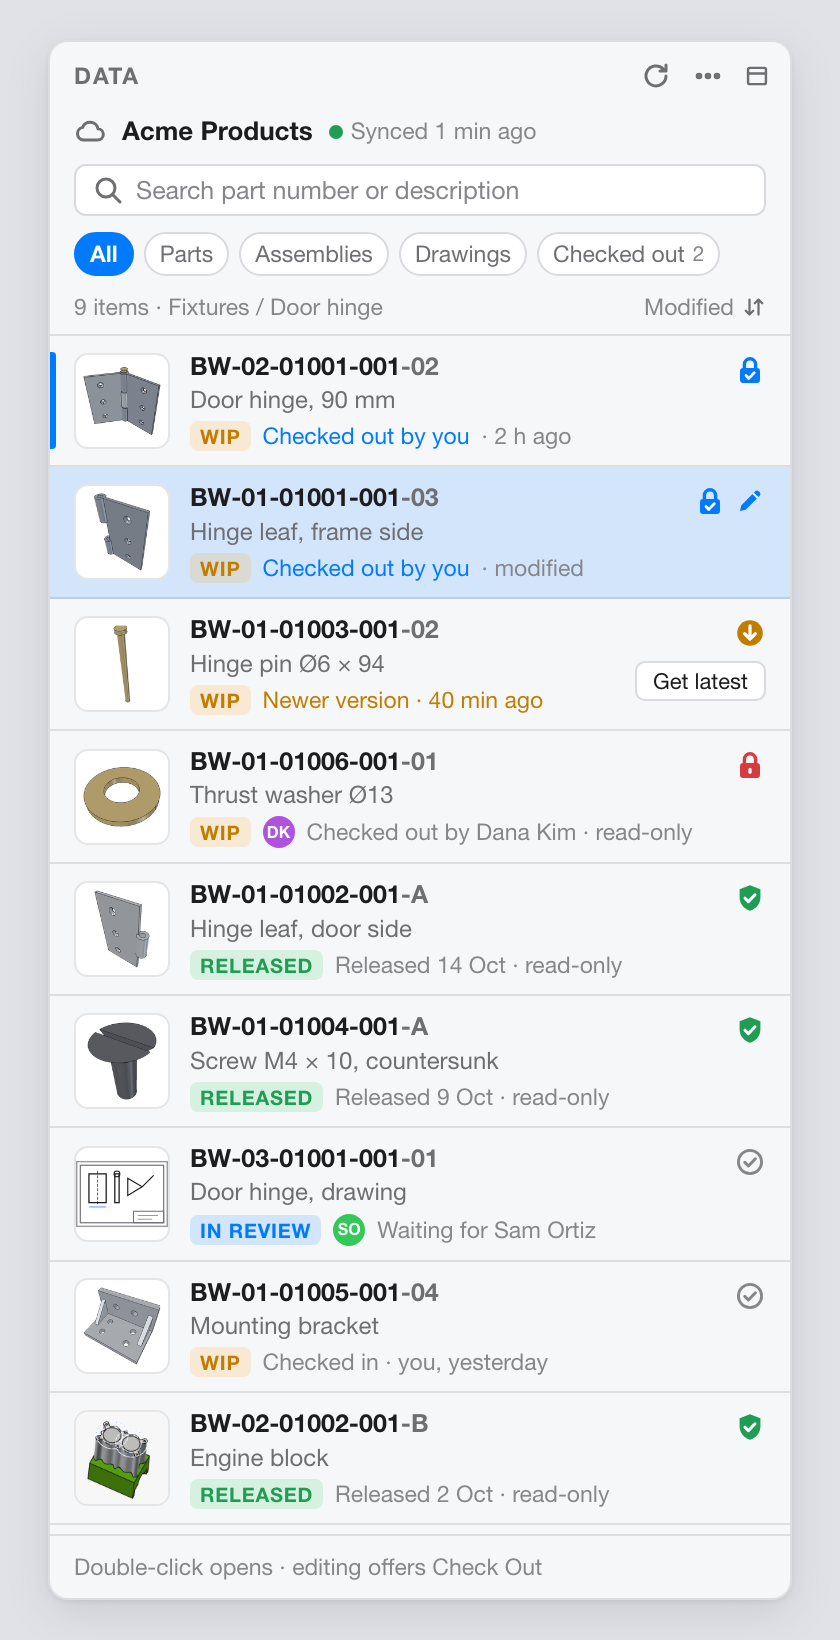
\includegraphics[width=0.48\linewidth]{fig/pdm04_datapanel.png}}{\fbox{pdm04\_datapanel.png}}\hfill
\IfFileExists{fig/pdm04_datapanel_dark.png}{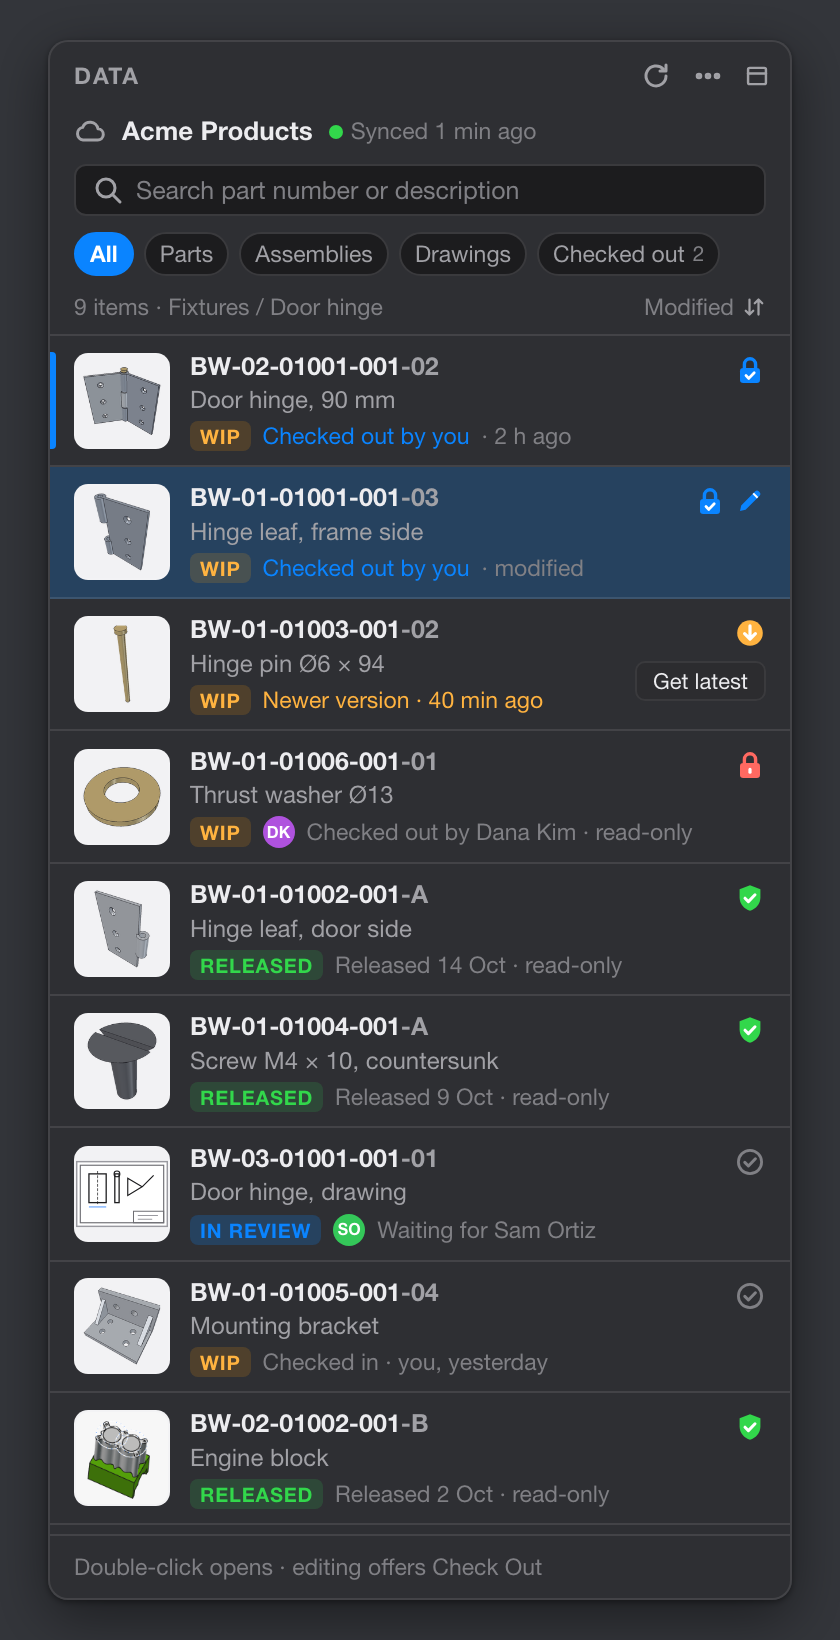
\includegraphics[width=0.48\linewidth]{fig/pdm04_datapanel_dark.png}}{\fbox{pdm04\_datapanel\_dark.png}}
\caption{The Data panel (mock), light and dark.}
\label{fig:pdm04-data}
\end{figure}

%----------------------------------------------------------------------
\subsubsection*{6. Build order and effort}

\begin{center}
\small
\begin{tabularx}{\linewidth}{@{}lXl@{}}
\toprule
\# & Step & Effort\\
\midrule
1 & Start page: the one-line vault switcher and \emph{My work} (checked out to me, in review) & 0.5\,d\\
2 & Work folder, \file{state.json}, the status function and its cache; pure Python with tests & 1.5\,d\\
3 & Operations and the link rewrite (zip only), with FreeCADCmd smoke tests on copies of the checklist files & 2\,d\\
4 & Read-only files, the save prompt, opening read-only, the iCloud download request & 1\,d\\
5 & Data panel & 1.5\,d\\
6 & Browser badges and menu, status bar, \emph{newer versions} in My work & 1\,d\\
7 & \code{LE-02001} round trip from an iCloud Drive vault; checklist; write-up & 0.5\,d\\
\midrule
 & Total & 8\,d\\
\bottomrule
\end{tabularx}
\end{center}
\textbf{Risks.} A save refused by the file system may leave FreeCAD in an odd state (checked first, step~4; the
fallback is to cancel the save through the Std\_Save command instead). Very large assemblies make the first status
pass slow until the hash cache is warm. The PySide clean-up found in the vault task panels applies to the new panels
too. No upstream conflict: everything is Python except, possibly, a \code{[BW]} hook if step~4 needs one.

%----------------------------------------------------------------------
\subsubsection*{Your answers (23 Oct, evening)}
Recommendations 1, 5 and 6 accepted (fetch linked parts at once; Submit and Approve now; the panel is called
\emph{Vault}). Changed: \textbf{a check-in comment is required} (OK stays disabled until there is one), and
\textbf{no backup files} for vault files: every check-in is a version, and FreeCAD's own crash recovery, which
lives outside iCloud, covers the time between check-ins. Stale locks: no expiry; \emph{Break lock\ldots} in Vault
Settings. Because the actor name is \code{user@mac} and macOS sometimes renames the Mac (``-2'' after a name
clash), the client \textbf{pins the actor} the first time it opens a vault, so a rename never orphans your own
locks. One Mac is assumed until much later.

%----------------------------------------------------------------------
\subsubsection*{Built (24 Oct 2026)}
The vault client (\file{bruceworx\_vaultclient.py}: commands, Check In panel, Vault panel, Browser badges, status
bar, save prompt, Move vault) was built on 23 Oct. On 24 Oct the rest of the plan was added:
\begin{itemize}[nosep]
  \item \textbf{Links on check-in} (\S4). Before a check-in, \code{Workspace.fix\_links} reads every link in the
        files going in. A link that is already \file{<P/N>.FCStd} is left alone. A link to a vault file by some other
        path (another work folder, an imported original, a copy with the same content) is pointed at its part number.
        A file that is not in the vault yet is shown in the panel's \emph{Links} box with ``Import it into the vault
        with a new part number and link to it'' (ticked): it is imported with what it links in turn
        (\code{vault\_setup.import\_linked\_files}, numbers from the program of the item being checked in), and the
        links are rewritten in the zip before the file goes to \file{objects/}. Unticked, or for a file that cannot be
        found, the link goes in as written and the box says so. An open document whose links changed is read again,
        so a later save cannot write the old paths back.
  \item \textbf{Import fixes.} The Create Vault import now numbers parts before the assemblies that link them (it went
        in file-name order, so \file{a-frame.FCStd} kept its old links), and it drops the ``Link not restored'' error
        FreeCAD saved in the copy it numbered, which showed as \textsc{error} on every link in the Browser.
  \item \textbf{iCloud: download before open} (\S1). \code{needs\_download} spots a file iCloud keeps only in the
        cloud: \emph{dataless} on macOS~14 and later (\code{st\_flags} has \code{SF\_DATALESS}), or replaced by a
        \file{.<name>.icloud} stand-in on older macOS. Before the workspace reads a vault object or a work file
        (check out, get latest, get revision, check in, open with everything it links), it asks for the download
        through \code{NSFileManager startDownloadingUbiquitousItemAtURL:error:} (ctypes, as for the Trash) and waits
        with a progress dialog (``Downloading 2 files (14 MB) from iCloud\ldots'', Cancel). If no file arrives for
        2~minutes it stops with ``\ldots{} did not download from iCloud \ldots{} Check that this Mac is online and
        signed in to iCloud''. Status passes never read an evicted file: its hash is kept in \file{state.json}.
  \item \textbf{Tests.} Add-on: \file{test\_pdm\_workspace.py} (stand-ins, dataless files, waits, time-outs, status
        without reading) and \file{test\_vault\_links.py} (check-in links: import, by path, same content, missing
        file, sub-assemblies); FreeCAD: \code{TestBruceWorxVaultClient}, \code{TestBruceWorxVaultWizard},
        \code{TestBruceWorxStart} pass.
\end{itemize}

\begin{figure}[!htbp]
\centering
\IfFileExists{fig/pdm04_built_checkin.png}{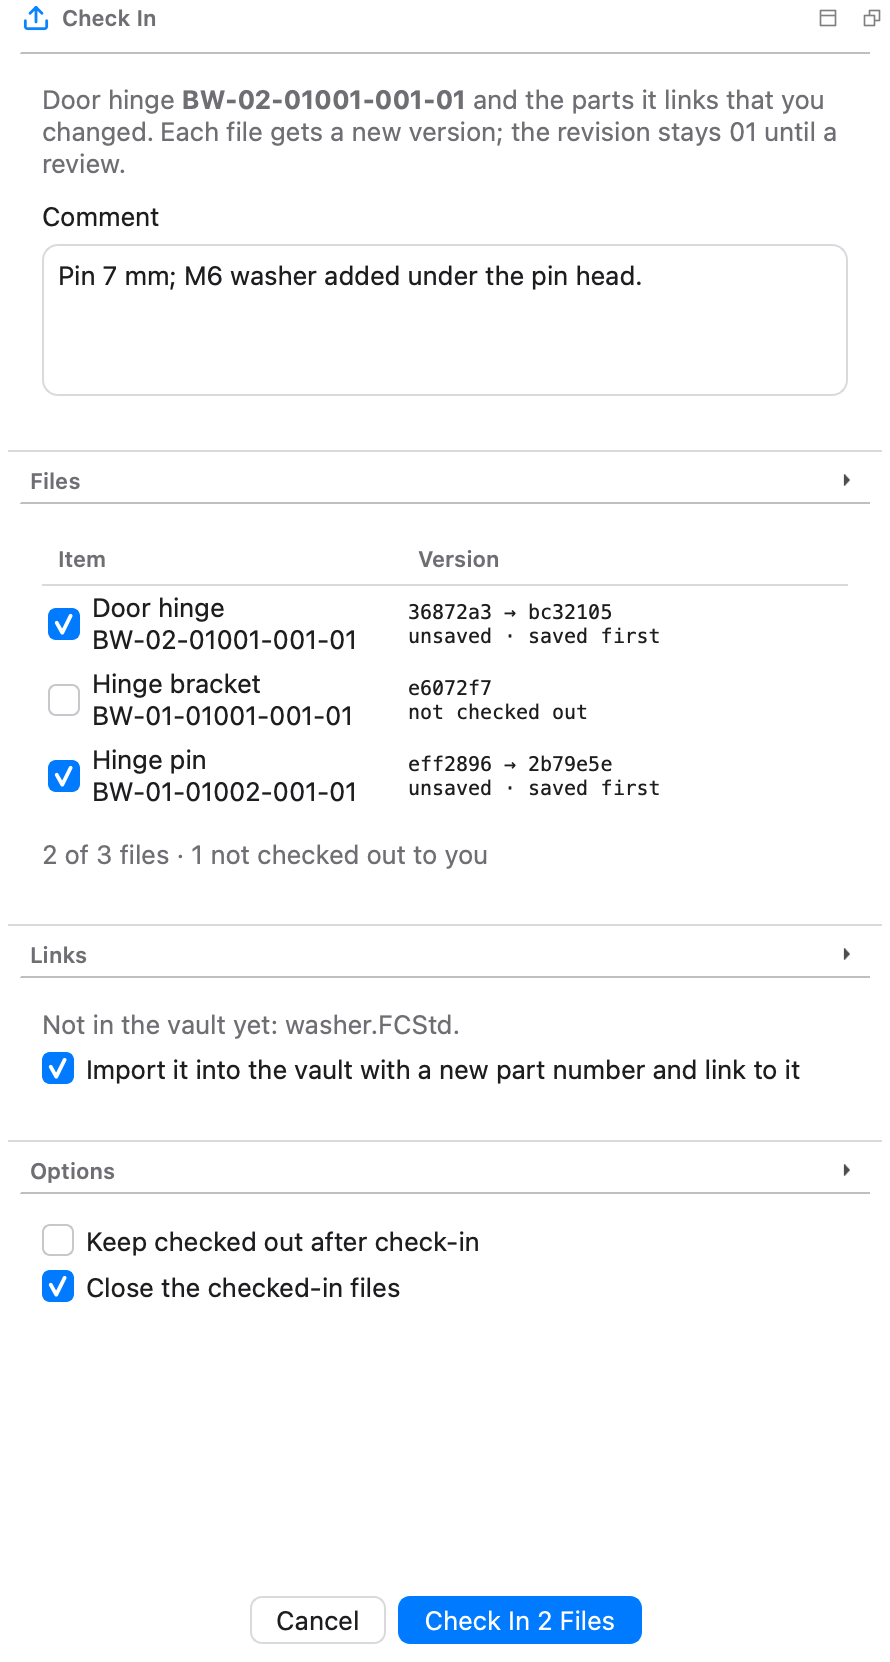
\includegraphics[height=8.5cm]{fig/pdm04_built_checkin.png}}{\fbox{pdm04\_built\_checkin.png}}\hspace{6mm}
\IfFileExists{fig/pdm04_built_states.png}{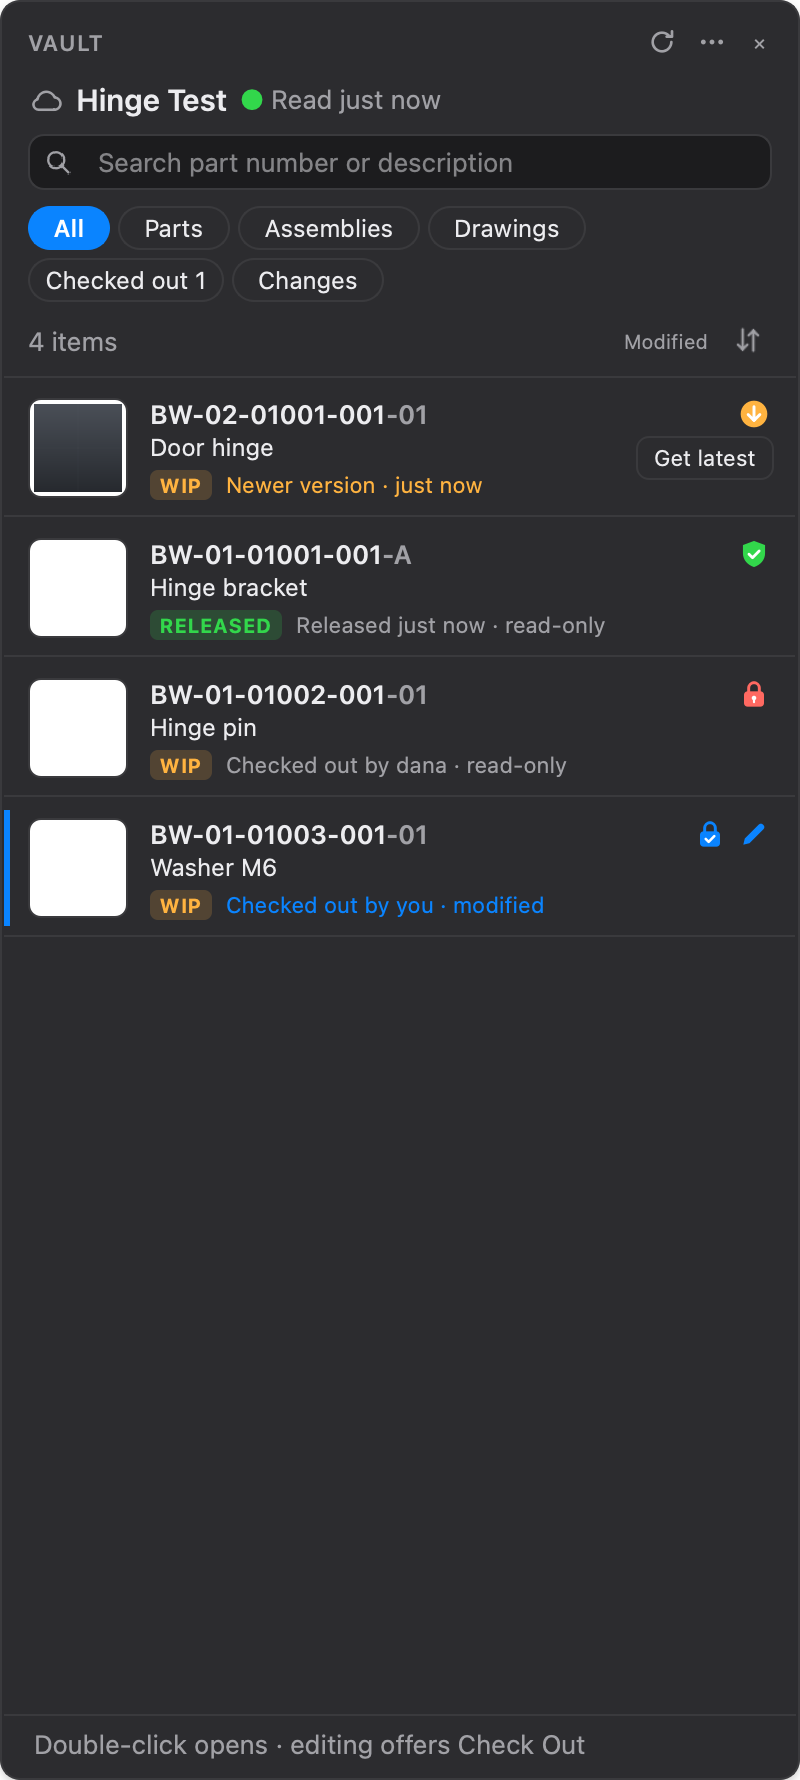
\includegraphics[height=8.5cm]{fig/pdm04_built_states.png}}{\fbox{pdm04\_built\_states.png}}
\caption{As built. \emph{Left:} Check In with a washer linked from outside the vault (light). \emph{Right:} the Vault
panel showing newer, released, checked out by someone else and checked out to you, modified (dark).}
\label{fig:pdm04-built}
\end{figure}

\paragraph{Your answers to the two questions left by the build (24 Oct).}
\begin{center}
\small
\begin{tabularx}{\linewidth}{@{}>{\raggedright\arraybackslash}p{5.6cm}X@{}}
\toprule
Question & Answer\\
\midrule
\emph{File $\rightarrow$ Open} and \emph{Open Recent} on a vault file go straight to FreeCAD, past the client, so an
  evicted iCloud file blocks with no progress dialog. Should they go through the client? & \textbf{Yes}: both go
  through the vault client, which downloads first (with its progress dialog) and opens the file as the Vault panel
  does.\\
After an import at check-in, the outside original (e.g.\ \file{washer.FCStd}) stays where it was. Offer to move it to
  the Trash? & \textbf{No}: originals of imported outside files stay where they are; no Trash offer.\\
\bottomrule
\end{tabularx}
\end{center}

\paragraph{Acceptance, to repeat on LE-02001.} Run in a scratch vault (not in iCloud Drive) on a door hinge assembly
linking a bracket and a pin, light and dark, through the client: 27 checks, all passed. The iCloud download was
simulated with \file{.icloud} stand-ins; a real iCloud Drive vault is the step still to do. The same steps on
\code{LE-02001}:
\begin{enumerate}[nosep]
  \item Create a vault in iCloud Drive (Start page $\rightarrow$ Create vault) and import the folder that holds
        \code{LE-02001} and its parts. Open the Vault panel (click ``Vault \ldots'' in the status bar): every row
        reads \emph{Checked in, up to date}.
  \item Right-click the assembly $\rightarrow$ \emph{Check Out}, then double-click it. It opens with all its parts;
        the parts' tabs show a lock and the Browser shows ``WIP 01'' and a lock on the assembly.
  \item Change a part you checked out too, and add a part from outside the vault to the assembly. Save. Both rows read
        \emph{Checked out to me, modified}.
  \item \emph{Check In\ldots} (Shift-Cmd-I): write a comment; the \emph{Links} box offers to import the outside
        part. Check in. The new part has a P/N, every row is up to date and read-only, and the assembly reopens with
        no broken links.
  \item On a second Mac (or from the command line as another user) check in a change to a part: its row turns
        \emph{Newer} with \emph{Get latest}; click it. Then, in Finder, \emph{Remove Download} on the assembly and
        open it from the Vault panel: the download dialog appears and the file opens.
\end{enumerate}

%----------------------------------------------------------------------
\subsubsection*{Questions before PDM-04 starts}

\begin{enumerate}
  \item \textbf{Checking out an assembly.} Fetch everything it links to (read-only) at once, or only when the
        assembly is opened?\\
        \emph{Recommendation:} at once, so the assembly always opens complete; it costs only disk space.
  \item \textbf{Check-in comment.} Required, or optional with a default (``Checked in from FreeCAD'')?\\
        \emph{Recommendation:} optional; a release (\eref{PDM-05}) will require one.
  \item \textbf{Stale locks.} One writer at a time means a lock is only stale after a crash or a lost Mac. Expire
        locks after some days, or only let Vault Settings break a lock?\\
        \emph{Recommendation:} no expiry; \emph{Break lock\ldots} in Vault Settings, recorded in the journal.
  \item \textbf{Backups of work files.} Keep FreeCAD's backups (moved to \file{.bw/backup/}, one per file), or
        turn them off for vault files since every check-in is a version anyway?\\
        \emph{Recommendation:} keep one, moved; it covers a crash between check-ins.
  \item \textbf{Submit and approve.} The vault model already has them. Add \emph{Submit for review} and
        \emph{Approve} to the menus now (one user approves their own work), or leave all lifecycle actions to
        \eref{PDM-05}?\\
        \emph{Recommendation:} add both now so \code{LE-02001} can reach rev A; ECR and ECO stay in PDM-05.
  \item \textbf{The panel's name.} Fusion calls it the \emph{Data} panel, but FreeCAD's property editor already
        has a \emph{Data} tab, so ``Data'' would mean two things. Call it \emph{Data} anyway, or \emph{Vault}?\\
        \emph{Recommendation:} \emph{Vault}.
\end{enumerate}
